\maketitle

Due: Wednesday, April 17 at 11:59 pm.

\section{Practice problems -- do not submit}
\subsection{13.1. Vector fields}
\begin{practice}p.1059 \#1\end{practice}
\begin{pracsol}
  This is a constant vector field. All vectors are parallel and have the same length and direction. See the picture below.
  \begin{center}
    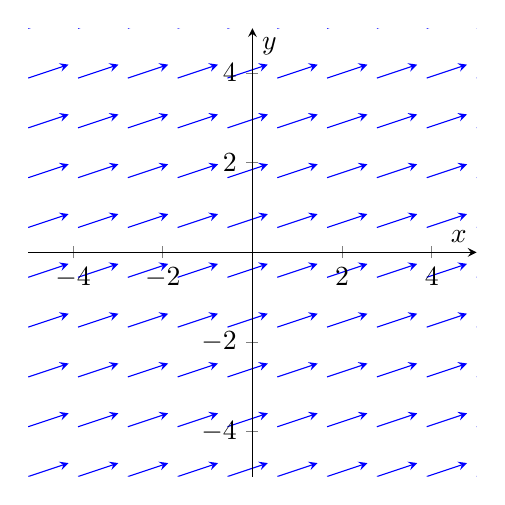
\begin{tikzpicture}
      \begin{axis}[axis lines=middle, axis equal image, xmin=-5, xmax=5, ymin=-5, ymax=5, zmin=0, zmax=1, xlabel=$x$, ylabel=$y$, view={0}{90}]
        \addplot3[blue, quiver={u={3},v={1}, scale arrows=0.3}, -stealth, domain=-5:5, domain y=-5:5, samples=10] {0};
      \end{axis}
    \end{tikzpicture}
  \end{center}
\end{pracsol}
\begin{practice}p.1059 \#8\end{practice}
\begin{pracsol}
  \begin{center}
    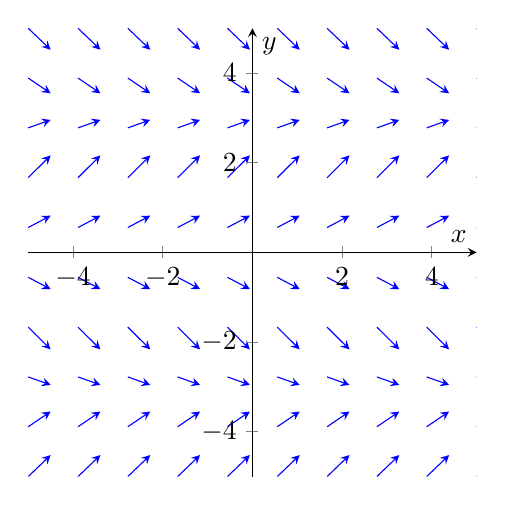
\begin{tikzpicture}
      \begin{axis}[axis lines=middle, axis equal image, xmin=-5, xmax=5, ymin=-5, ymax=5, zmin=0, zmax=1, xlabel=$x$, ylabel=$y$, view={0}{90}]
        \addplot3[blue, quiver={u={1},v={sin(deg(y))}, scale arrows=0.5}, -stealth, domain=-5:5, domain y=-5:5, samples=10] {0};
      \end{axis}
    \end{tikzpicture}
  \end{center}
\end{pracsol}
\begin{practice}p.1059 \#9\end{practice}
\begin{pracsol}
  The direction of the field at any point $P=(x,y,z)$ is the $\bj$ vector. Since the magnitude of the field is $\|\mathbf F(P)\|=\alpha\sqrt{x^2+z^2}$ (here, $\alpha$ is the proportionality constant), $\mathbf F(x,y,z)=\alpha\sqrt{x^2+z^2}\bj$.  (The domain of the vector field is $-4<x<4,0<z<10$.)
\end{pracsol}
\begin{practice}p.1059 \#12\end{practice}
\begin{pracsol}
  The orientation implies that the rotation is clockwise when viewed in the usual axes we have been using. The $y$-coordinate of the input has no bearing on the output, and the $y$-coordinate of the output is 0. Therefore the direction of the vector field at $(x,y,z)$ is parallel to either $(z,0,-x)$ or $(-z,0,x)$. We find (e.g.\ by testing positive $z$ and $x=0$) that $(z,0,-x)$ gives the clockwise direction. Finally, we need the vector field's output to have magnitude $\alpha(x^2+z^2)$, but $(z,0,-x)$ already has magnitude $\sqrt{x^2+z^2}$, so we have to multiply $(z,0,-x)$ by an additional factor of $\alpha\sqrt{x^2+z^2}$. Our formula is
  \[\mathbf F(x,y,z)=\alpha\sqrt{x^2+z^2}(z\bi-x\bk).\]
\end{pracsol}
\begin{practice}p.1060 \#19\end{practice}
\begin{pracsol}
  $\nabla u(x,y,z)=((x-y)\ln(z))^{-1}\bi-((x-y)\ln(z))^{-1}\bj-\frac{\ln(x-y)}{z \ln^2(z)}\bk$.
\end{pracsol}
\begin{practice}p.1060 \#25\end{practice}
\begin{pracsol}
  We need $u_x(x,y)=y^3+2xy$, so $u(x,y)$ is of the form $xy^3+x^2y+g(y)$. Then $u_y(x,y)=3xy^2+x^2+g'(y)$ and must be equal to $3xy^2+x^2$, so $g'(y)=0$ and $g(y)$ is a constant. We can set $g(y)=0$, to get $u(x,y)=xy^3+x^2y$.
\end{pracsol}
\begin{practice}p.1060 \#38\end{practice}
\begin{pracsol}
  Let $\br(t)=(x(t),y(t))$. We need to solve the differential equations $x'(t)=1,y'(t)=-x(t)$. The first one has solution $x(t)=t+C$, and plugging this into the second equation gives $y'(t)=-t-C\implies y(t)=-\frac12t^2-Ct+D$. So
  \[\br(t)=\left(t+C,-\frac12t^2-Ct+D\right).\]
\end{pracsol}

\subsection{13.2. Line integrals}
\begin{practice}p.1070 \#1\end{practice}
\begin{pracsol}
  Observe that $\mathbf F(\br(t))=(\cos(t)\sin(t),\sin^2(t))$ and $\br'(t)=(-\sin(t),\cos(t))$. Therefore, $\mathbf F(\br(t))\cdot\br'(t)=-\cos(t)\sin^2(t)+\sin^2(t)\cos(t)=0$, and
  \[\int_{\mathcal C}\mathbf F\cdot d\br=\int_0^{\frac{\pi}{3}}\mathbf F(\br(t))\cdot\br'(t)\,dt=\int_0^{\frac\pi3}0\,dt=0.\]
\end{pracsol}
\begin{practice}p.1070 \#14\end{practice}
\begin{pracsol}
  We just calculate
  \[\begin{split}
    \int_{\mathcal C}\mathbf F\cdot d\br &= \int_0^{2\pi}\mathbf F(\sin(t),\cos(t),\sin(t))\cdot (\cos(t),-\sin(t),\cos(t))\,dt\\
    &= \int_0^{2\pi}(\cos(t),\sin(t)-\sin(t),\sin(t))\cdot (\cos(t),-\sin(t),\cos(t))\,dt\\
    &= \int_0^{2\pi}(\cos^2(t)+\sin(t)\cos(t))\,dt\\
    &=\pi.
  \end{split}\]
\end{pracsol}
\begin{practice}p.1070 \#23\end{practice}
\begin{pracsol}
  Using formula (15.20) with $x(t)=t^2,y(t)=t^3,z(t)=t^4$,
  \[\begin{split}
    \int_{\mathcal C}\mathbf F\cdot d\br &= \int_{\mathcal C}xz\,dx+yz\,dy+xy\,dz\\
    &= \int_0^1\left((t^2\cdot t^4)x'(t)+(t^3\cdot t^4)y'(t)+(t^2\cdot t^3)z'(t)\right)\,dt\\
    &= \int_0^1 (t^6(2t)+t^7(3t^2)+t^5(4t^3))\,dt\\
    &= \int_0^1 (2t^7+3t^9+4t^8)\,dt\\
    &= \frac{179}{180}.
  \end{split}\]
\end{pracsol}

\newpage

\section{Homework problems -- submit these}

\begin{problem}
  The given vector fields are conservative. Find a potential function for each. You can use any method you like, including guess and check.
  \begin{enumerate}[(a)]
    \item $2e^{2x-y}\bi-e^{2x-y}\bj$
    \begin{solution}
      We seek $(x,y)\mapsto u(x,y)$ such that $(u_x,u_y)=(2e^{2x-y},-e^{2x-y})$. The equation $u_x=2e^{2x-y}$ implies that $u(x,y)=\int 2e^{2x-y}\,dx+\phi(y)=e^{2x-y}+\phi(y)$ for some scalar-valued function of one variable $\phi(y)$. Differentiating this with respect to $y$ then yields $u_y(x,y)=-e^{2x-y}+\phi'(y)$. Matching this with $-e^{2x-y}$ (from the first line) we see that $\phi'(y)$ must be 0. We can set $\phi(y)=0$, to get the potential function
      \[u(x,y)=e^{2x-y}.\]
    \end{solution}
    \item $\left(\ln(x+y)+\frac{x}{x+y}\right)\bi+\frac{x}{x+y}\bj$
    \begin{solution}
      We seek $(x,y)\mapsto u(x,y)$ such that $(u_x,u_y)=\left(\ln(x+y)+\frac{x}{x+y},\frac{x}{x+y}\right)$. This time the $y$-component looks like the simpler thing to take the antiderivative of. So solving $u_y=\frac{x}{x+y}$ yields $u=\int \frac{x}{x+y}\,dy+\phi(x)=x\ln(x+y)+\phi(x)$ for some scalar-valued function $\phi(x)$. Differentiating this with respect to $x$ we then get $u_x=\ln(x+y)+\frac{x}{x+y}+\phi'(x)$. Matching this with $\ln(x+y)+\frac{x}{x+y}$ (from the first line) we get that $\phi'(x)$ must be 0, so we can set $\phi(x)=0$ to get
      \[u(x,y)=x\ln(x+y).\]
      It is also possible to solve this by antidifferentiating $u_x$ with respect to $x$ as the first step, just a lot more complicated. Just for fun, here's how it goes:
      \[\begin{split}
        u &= \int\left(\ln(x+y)+\frac{x}{x+y}\right)\,dx+\phi(y)\\
        &= \int\ln(x+y)\,dx+\int\frac{x}{x+y}\,dx+\phi(y)\\
        &= \int\ln(x+y)\,dx+\int\left(1-\frac{y}{x+y}\right)\,dx+\phi(y)\\
        &= \left((x+y)\ln(x+y)-(x+y)\right)+\left(x-y\ln(x+y)\right)+\phi(y)\\
        &= x\ln(x+y)-y+\phi(y).
      \end{split}\]
      Then $u_y=\frac{x}{x+y}-1+\phi'(y)$ which we must match with $\frac{x}{x+y}$, so $\phi'(y)$ must equal 1 and so we can set $\phi(y)=y$, to get $u=x\ln(x+y)$. It is interesting that we get a nontrivial $\phi(y)$ in this case.
    \end{solution}
  \end{enumerate}
\end{problem}

\begin{problem}
  Coulomb's law says that the force $\mathbf F$ acting on a charge $q$ at position $\mathbf r$ because of a charge $Q$ at the origin is
  \[\mathbf F=\frac{\eps Qq}{\|\br\|^3}\br,\]
  where $\eps$ is a positive constant that depends on the physical units used.
  \begin{enumerate}[(a)]
    \item Show that $V=\frac{\eps Qq}{\|\br\|}$ is a potential function for $\mathbf F$.
    \begin{solution}
      We show that (physics convention) $\nabla V=-\BF$, by direct calculation. First, write $\br$ as $(x,y,z)$, so that
      \[V(x,y,z)=\frac{\eps Qq}{\sqrt{x^2+y^2+z^2}}=\eps Qq(x^2+y^2+z^2)^{-\frac12}.\]
      Then
      \[\begin{split}
        \nabla V &= \eps Qq \left(2x\cdot-\frac12(x^2+y^2+z^2)^{-\frac32},2y\cdot-\frac12(x^2+y^2+z^2)^{-\frac32}\right.\\
        &\qquad\qquad \left.2z\cdot-\frac12(x^2+y^2+z^2)^{-\frac32}\right)\\
        &= -\eps Qq(x^2+y^2+z^2)^{-\frac32}(x,y,z)\\
        &= -\eps Qq\|\br\|^{-3}\|\br\|\\
        &= -\BF.
      \end{split}\]
    \end{solution}
    \item If $Qq>0$, then $\mathbf F$ is said to be \emph{repulsive}, while if $Qq<0$, then $\mathbf F$ is said to be \emph{attractive}. Explain why this terminology is appropriate.
    \begin{solution}
      When $Qq>0$, the direction of $\BF$ is parallel to $\br$ and in the same direction as $\br$, meaning the force field points outwards away from the origin. This represents a repulsive force.

      When $Qq<0$, the direction of $\BF$ is parallel to $\br$ but in the opposite direction of $\br$, meaning the force field points inwards toward the origin. This represents an attractive force.
    \end{solution}
  \end{enumerate}
\end{problem}

\begin{problem}
  At the point $(x,y)$, the elevation of the terrain is $h(x,y)=-x^2+3xy+2y^2+100$ feet. Sketch the vector field that shows the direction of quickest descent at each point.
\end{problem}
\begin{solution}
  The vectors in this field are negatives of the gradient vectors for the function $h$:
  \[\BF(x,y) = -\nabla h(x,y)=(2x-3y)\bi+(-3x-4y)\bj.\]
  See the picture below.
  \begin{center}
    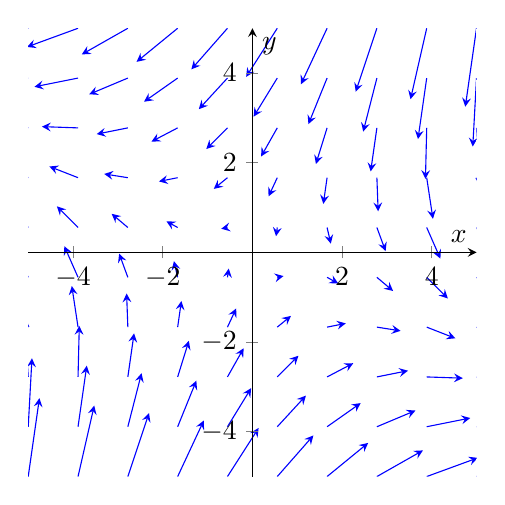
\begin{tikzpicture}
      \begin{axis}[axis lines=middle, axis equal image, xmin=-5, xmax=5, ymin=-5, ymax=5, zmin=0, zmax=1, xlabel=$x$, ylabel=$y$, view={0}{90}]
        \addplot3[blue, quiver={u={2*x-3*y},v={-3*x-4*y}, scale arrows=0.05}, -stealth, domain=-5:5, domain y=-5:5, samples=10] {0};
      \end{axis}
    \end{tikzpicture}
  \end{center}
\end{solution}

\begin{problem}
  Show that $F(x,y)=y\bi+2x\bj$ is not the gradient vector field of any continuously differentiable function.
\end{problem}
\begin{solution}
  If there were a continuously differentiable function $(x,y)\mapsto u(x,y)$ such that $\nabla u(x,y)=(y,2x)$, then $u_x(x,y)=y$ and $u_y(x,y)=2x$. There are some ways to proceed from here:
  \begin{itemize}
    \item If we make the additional assumption that $u$ is twice continuously differentiable, then we can check the mixed partials, which we know must agree for any twice continuously differentiable function: $u_{xy}(x,y)=1$ and $u_{yx}(x,y)=2$. These don't agree, which is a contradiction.

    Note that this is another way of stating the curl test (closed vector field test) from Section 13.3 (which you might have seen if you read ahead). The curl test is the test that $M_y=N_x$, if the vector field is of the form $(M,N)$.
    \item If we don't make this assumption, we can still proceed as follows: the equation $u_x(x,y)=y$ implies that $u(x,y)=\int y\,dx+\phi(y)=xy+\phi(y)$ for some scalar-valued function $\phi$. Differentiating this with respect to $y$ we get that $u_y(x,y)=x+\phi'(y)$, which must equal $2x$. So $\phi'(y)=2x-x=x$, which is impossible since $\phi'(y)$ cannot depend on $x$.
  \end{itemize}
\end{solution}

\begin{problem}
  How difficult was each problem? Rate each problem (and part) on a difficulty scale from 1 to 7, where 1 means ``super easy, barely an inconvenience!'' and 7 means ``hardest problem I've ever done.''
\end{problem}
